\PassOptionsToPackage{table,dvipsnames,svgnames}{xcolor}
\documentclass[11pt, twoside, a4paper]{report}
\usepackage[inner = 30mm, outer = 20mm,  top = 30mm, bottom = 20mm, headheight = 13.6pt]{geometry}
\usepackage{tikz}
\usepackage[pdfpagelayout=TwoPageRight]{hyperref}
\usepackage[export]{adjustbox}
%\usepackage{showframe}
\hypersetup{colorlinks=true, linktoc=all, allcolors=green!30!black,}

\usepackage{calc}
\usepackage{ifthen}
\usepackage{pgfplots}
\usepackage{siunitx}

\immediate\write18{if not exist tikz_external mkdir tikz_external} % Only tested on Windows

\usepgfplotslibrary{external}
\tikzexternalize[
    prefix={./},
    only named,
]
\usetikzlibrary{arrows.meta}
\usetikzlibrary{math}
\usetikzlibrary{patterns}
\usetikzlibrary{decorations.pathmorphing,decorations.markings}

% Make the 'export as png' a seperate style, with default density 200
\tikzset{
    export as png/.style={
        external/system call/.add={}{
            && convert -density #1 -transparent white "\image.pdf" "\image.png"
        },
    },
    export as png/.default={600},
}

\pgfmathdeclarerandomlist{MyRandomColors}{%
    {red}%
    {magenta}%
    {olive}%
    {brown}%
    {violet}%
    {gray}%
    {purple}%
    {yellow}%
    {orange}%
    {cyan}%
    {green}%    
}%

\begin{document}

  \begin{center}
    \tikzset{export as png}
    \tikzsetnextfilename{squares}
    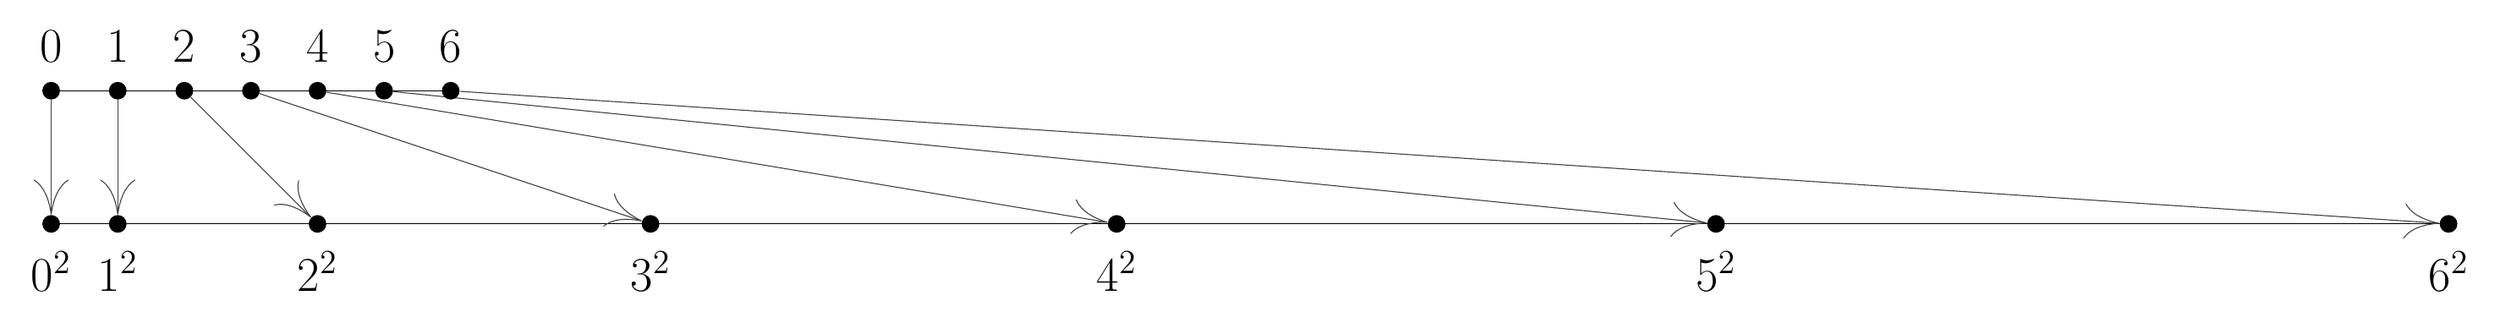
\begin{tikzpicture}
      \draw (0,2) -- (6,2);
      \draw (0,0) -- (36,0);
      \foreach \i in {0,1,2,3,4,5,6} {
        \node[circle,fill=black,minimum size=0.3mm,scale=0.8] (num\i) at (\i, 2) {};
        \node[circle,fill=black,minimum size=0.3mm,scale=0.8] (square\i) at ({\i^2}, 0) {};
 
        \draw (\i, 2.3) node[above] {\huge $\i$};
        \draw ({\i^2}, -0.3) node[below] {\huge $\i^2$};
 
        \draw[darkgray,-{>[scale=5,
                           length=3,
                           width=3]}] (num\i) -- (square\i);
      }
    \end{tikzpicture}
  \end{center}

  \begin{center}
    \tikzset{export as png}
    \tikzsetnextfilename{sqroots}
    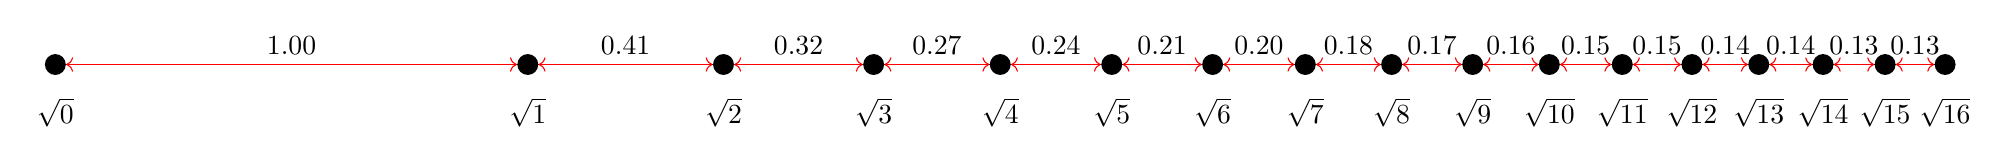
\begin{tikzpicture}[scale=6]
      \draw (0,0) -- (4,0);
      \foreach \i in {0,...,16} {
        \node[circle,fill=black,minimum size=0.3mm,scale=0.8] (sqroot\i) at ({sqrt(\i)}, 0) {};

        \draw ({sqrt(\i)}, -0.3/6) node[below] {$\sqrt{\i}$};
        \ifthenelse{\i > 0}{
          \tikzmath{
            \lasti = \i - 1;
            \dist = sqrt(\i) - sqrt(\lasti);
          }
          \draw[<->,red] (sqroot\lasti) -- (sqroot\i);
          \path (sqroot\lasti) -- (sqroot\i) node[midway,above] (b)
          {$\num[round-mode=places,round-precision=2]{\dist}$};
        }{}
      }
    \end{tikzpicture}
  \end{center}

  \begin{center}
    \tikzset{export as png}
    \tikzsetnextfilename{sqroot-4-to-9}
    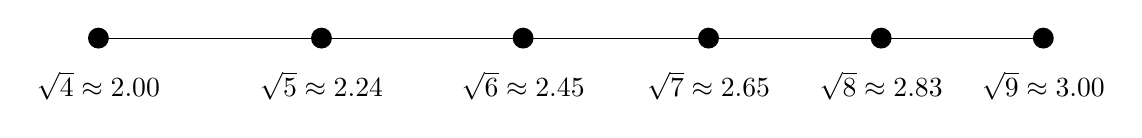
\begin{tikzpicture}[scale=12]
      \draw (2,0) -- (3,0);
      \foreach \i in {4,...,9} {
        \node[circle,fill=black,minimum size=0.3mm,scale=0.8] (sqroot\i) at ({sqrt(\i)}, 0) {};

        \tikzmath{ \val = sqrt(\i); }
        \draw ({sqrt(\i)}, -0.3/12) node[below] {$\sqrt{\i} \approx
          \num[round-mode=places,round-precision=2]{\val}$};
      }
    \end{tikzpicture}
  \end{center}

%  \begin{center}
%    \tikzset{export as png}
%    \tikzsetnextfilename{sqroot-plot}
%    \begin{tikzpicture}
%      \draw[->,darkgray] (-1,0) -- (16 + 1,0) node[right] {$x$};
%      \draw[->,darkgray] (0,-1) -- (0,5) node[above] {$y$};
%      \draw[domain=0:16,smooth,samples=1000,variable=\x, gray] plot ({\x},{sqrt(\x)});
%      \foreach \i in {1,...,16} {
%        \pgfmathsetmacro{\pi}{\i-0.5}
%        \pgfmathsetmacro{\ni}{\i+0.5}
%        \pgfmathrandomitem{\RandomColor}{MyRandomColors} 
%
%        \draw[domain=\pi:\ni,smooth,samples=100,variable=\x,\RandomColor] plot ({\x},{1/(2*sqrt(\i)) * \x + sqrt(\i) - \i/(2*sqrt(\i))});
%      }
%    \end{tikzpicture}
%  \end{center}

%  \begin{center}
%    \tikzset{export as png}
%    \tikzsetnextfilename{square-plot}
%    \begin{tikzpicture}
%      \draw[->,darkgray] (-1,0) -- (4 + 1,0) node[right] {$x$};
%      \draw[->,darkgray] (0,-1) -- (0,16 + 1) node[above] {$y$};
%      \draw[domain=0:4,smooth,variable=\x,gray] plot ({\x},{\x^2});
%      \foreach \i in {1,...,4} {
%        \pgfmathsetmacro{\pi}{\i-0.5}
%        \pgfmathsetmacro{\ni}{\i+0.5}
%        \pgfmathrandomitem{\RandomColor}{MyRandomColors} 
%
%        \draw[domain=\pi:\ni,smooth,samples=100,variable=\x,\RandomColor] plot ({\x},{2*\i * \x +
%          \i^2 - \i*2*\i});
%      }
%    \end{tikzpicture}
%  \end{center}

  \begin{center}
    \tikzset{export as png}
    \tikzsetnextfilename{sqroot-diff-plot}
    \begin{tikzpicture}
      \draw[->,darkgray] (-1,0) -- (16 + 1,0) node[right] {$x$};
      \draw[->,darkgray] (0,-1) -- (0,1 + 1) node[above] {$y$};
      \draw[domain=0:16,smooth,variable=\x,gray] plot ({\x},{sqrt(\x+1)-sqrt(\x)});
    \end{tikzpicture}
  \end{center}

\end{document}
